\documentclass[11pt,a4paper]{article}
\usepackage{amsmath, amssymb}
\usepackage{graphicx}
\usepackage[a4paper,margin=2.2cm]{geometry}
\usepackage{float}
\usepackage[indonesian]{babel}
\usepackage{hyperref}
\addto\captionsindonesian{
  \renewcommand{\figurename}{Gambar}
  \renewcommand{\tablename}{Tabel}
}

\title{\Huge {Analisis Representasi dan Spektrum Sinyal}\\
\Large{Tugas \textit{Case-Based} 1}}
\author{\Large{Junika Irdia Indi Astudin (6002261013)}\\
\Large{Teosofi Hidayah Agung (6002261009)}
}
\date{1 Oktober 2026}
% Fragmen tabel numerik dibaca tanpa menambahkan baris kosong.
\makeatletter
\let\inputrows\@@input
\makeatother
\newcommand{\EnergiInterval}{1.2528701371}
\newcommand{\EnergiParseval}{1.2528701369}
\newcommand{\GalatParseval}{$1.4537\times10^{-10}$}
\newcommand{\EnergiWaktu}{1.2528764176}
\newcommand{\EnergiFrekuensi}{1.2528764176}
\newcommand{\GalatPlancherel}{$6.6613\times10^{-16}$}
\newcommand{\GalatRelPlancherel}{$5.3168\times10^{-16}$}
\newcommand{\MaksSinus}{$3.5339\times10^{-17}$}
\newcommand{\BedaKoefisien}{$5.8348\times10^{-13}$}
\newcommand{\BedaEnergiInterval}{$2.4425\times10^{-15}$}
\newcommand{\GalatModulasi}{$1.1102\times10^{-16}$}
\newcommand{\BedaBatasWaktu}{$0.0000\times10^{0}$}
\newcommand{\BedaBatasSpektrum}{$0.0000\times10^{0}$}


\begin{document}

\maketitle

\section{Pendahuluan}
Sinyal yang diamati dapat memuat beberapa komponen utama dan gangguan
yang berosilasi lebih cepat. Pengamatan pada domain waktu memperlihatkan
bentuk keseluruhan sinyal, sedangkan representasi Fourier membantu
mengenali komponen-komponennya berdasarkan frekuensi dan kontribusi
energinya.
Dalam tugas ini, sinyal dibentuk oleh dua komponen utama
dan satu gangguan berfrekuensi tinggi yang memiliki selubung Gaussian,
sesuai formulasi Tugas \textit{Case-Based} 1.

Analisis dilakukan melalui representasi ortogonal, deret Fourier,
aproksimasi jumlah parsial, dan transformasi Fourier. Deret Fourier
digunakan untuk mengamati sinyal pada interval terbatas beserta
periodisasinya, sedangkan transformasi Fourier digunakan untuk
mengamati spektrum sinyal asli pada seluruh domain waktu.
Kesamaan Parseval dan teorema Plancherel menghubungkan kedua
representasi tersebut dengan energi pada domain waktu masing-masing.

Tujuan laporan ini adalah menghitung koefisien Fourier dan galat
aproksimasi, mengidentifikasi komponen utama serta gangguan pada
spektrum, menyelidiki pengaruh amplitudo gangguan, dan membandingkan
hasil perhitungan energi. Sesuai arahan revisi, integral koefisien,
transformasi, dan energi dievaluasi secara numerik menggunakan
aturan Simpson komposit. Tabel dan grafik digunakan untuk
menjelaskan hasil serta waktu ketika komponen frekuensi tertinggi
memiliki amplitudo paling besar.

\section{Permasalahan}
Diberikan sinyal
\[
 f(t)=e^{-t^2/2}\left[\cos(\omega_1t)+\frac12\cos(\omega_2t)
 +\varepsilon\cos(\omega_3t)\right],
\]
dengan $0<\omega_1<\omega_2\ll\omega_3$ dan $0<\varepsilon<1$.
Dua komponen pertama merupakan komponen utama sinyal, sedangkan komponen
ketiga merepresentasikan gangguan berfrekuensi tinggi. Sesuai parameter
pada soal, digunakan $\omega_1=2$, $\omega_2=5$, $\omega_3=50$, dan
$\varepsilon=0.2$, sehingga
\begin{equation}
 f(t)=e^{-t^2/2}\left[\cos(2t)+\frac12\cos(5t)+0.2\cos(50t)\right].
 \label{eq:sinyal}
\end{equation}
Untuk deret Fourier, sinyal diamati pada $[-\pi,\pi]$ dan diperiodisasi
menjadi fungsi berperiode $2\pi$. Untuk transformasi Fourier, digunakan
sinyal asli pada seluruh $\mathbb R$, tanpa periodisasi.

Analisis mengikuti empat tahapan tugas: representasi ortogonal dan
koefisien deret Fourier; aproksimasi dan konvergensi jumlah parsial;
transformasi Fourier dan spektrum; serta perbandingan energi menggunakan
Parseval dan Plancherel. Koefisien, galat, dan energi dihitung secara
numerik dengan aturan Simpson komposit. Grafik digunakan untuk
mengidentifikasi dua komponen utama, gangguan frekuensi tinggi, dan
pengaruh $\varepsilon$. Waktu ketika komponen frekuensi tertinggi paling
kuat juga ditentukan dari evaluasi numerik sinyal.

\section{Dasar Teori}
\subsection{Ruang $L^2$}\label{sub ruang L^2} \nocite{bahanajar_kuliah1-4}

Ruang $L^2[-\pi,\pi]$ terdiri atas fungsi $f$ yang memenuhi

$$
  \int_{-\pi}^{\pi}|f(t)|^2\,dt<\infty.
$$
Hasil kali dalam dan norma didefinisikan sebagai
\[
 \langle f,g\rangle=\int_{-\pi}^{\pi}f(t)\overline{g(t)}\,dt,
 \qquad
 \|f\|_2=\left(\int_{-\pi}^{\pi}|f(t)|^2\,dt\right)^{1/2}.
\]

\subsection{Sistem Ortogonal dan Deret Fourier} \label{sub sistem ortogonal}
Sistem trigonometri
$
  \{1,\cos(nt),\sin(nt)\}_{n=1}^{\infty}
$
merupakan sistem ortogonal pada $L^2[-\pi,\pi]$.
Deret Fourier suatu fungsi $f$ adalah

$$
  f(t)
  \sim
  \frac{a_0}{2}
  +
  \sum_{n=1}^{\infty}
  \left[
    a_n\cos(nt)+b_n\sin(nt)
    \right],
$$
dengan koefisien

$$
  a_0
  =
  \frac{1}{\pi}
  \int_{-\pi}^{\pi}f(t)\,dt,
  \quad
  a_n
  =
  \frac{1}{\pi}
  \int_{-\pi}^{\pi}f(t)\cos(nt)\,dt,
  \quad
  b_n
  =
  \frac{1}{\pi}
  \int_{-\pi}^{\pi}f(t)\sin(nt)\,dt.
$$
Untuk fungsi genap, berlaku
$
  b_n=0.
$ Sedangkan untuk fungsi ganjil, berlaku $a_0=0$ dan $a_n=0.$

\subsection{Proyeksi Ortogonal dan Aproksimasi Fourier} \label{proyeksi ortogonal}

Subruang Fourier orde $K$ didefinisikan sebagai
$$
  V_K
  =
  \operatorname{span}
  \{1,\cos t,\sin t,\ldots,\cos(Kt),\sin(Kt)\}.
$$
Jumlah parsial Fourier merupakan proyeksi ortogonal $f$ pada $V_K$,
$
  S_Kf=P_{V_K}f.
$
Sebagai proyeksi ortogonal, $S_Kf$ merupakan aproksimasi terbaik dalam $V_K$,
$$
  \|f-S_Kf\|_2
  \leq
  \|f-g\|_2,
  \qquad
  g\in V_K.
$$
Karena sistem trigonometri lengkap di $L^2[-\pi,\pi]$, akibatnya
$
  \lim_{K\to\infty}
  \|f-S_Kf\|_2
  =
  0.
$

\subsection{Transformasi Fourier} \label{sub transformasi fourier}
Transformasi Fourier yang digunakan adalah transformasi dengan normalisasi
uniter,
\begin{equation}
 \widehat f(\omega)=\frac1{\sqrt{2\pi}}
 \int_{-\infty}^{\infty}f(t)e^{-i\omega t}\,dt.
 \label{eq:konvensi}
\end{equation}
Untuk $f,g\in L^1(\mathbb R)$, $\alpha,\beta\in\mathbb C$, dan
$\omega_0\in\mathbb R$, sifat linearitas dan modulasi dinyatakan sebagai
\[
 \mathcal F\{\alpha f+\beta g\}=\alpha\widehat f+\beta\widehat g,
 \qquad
 \mathcal F\{e^{i\omega_0t}g(t)\}(\omega)=\widehat g(\omega-\omega_0).
\]
Pasangan transformasi yang diberikan pada soal adalah
\[
 g(t)=e^{-t^2/2}\quad\longleftrightarrow\quad
 \widehat g(\omega)=e^{-\omega^2/2}.
\]
Pasangan ini menjadi acuan untuk memahami bentuk dan pergeseran spektrum.
Dalam pembahasan, nilai transformasi dihitung melalui kuadratur numerik.
Magnitudo spektrum dinyatakan oleh $|\widehat f(\omega)|$, sedangkan
$|\widehat f(\omega)|^2$ menyatakan kerapatan energi pada domain frekuensi.

\subsection{Kesamaan Parseval dan Teorema Plancherel}\label{kesamaan parseval}

Untuk deret Fourier kompleks,
$
  \int_{-\pi}^{\pi}|f(t)|^2\,dt
  =
  2\pi
  \sum_{n\in\mathbb{Z}}|c_n|^2.
$
Dalam bentuk real,
$$
  \frac{1}{\pi}
  \int_{-\pi}^{\pi}|f(t)|^2\,dt
  =
  \frac{a_0^2}{2}
  +
  \sum_{n=1}^{\infty}
  \left(a_n^2+b_n^2\right).
$$
Transformasi Fourier mempertahankan norma $L^2$,
$
  \|f\|_2
  =
  \|\widehat{f}\|_2.
$
Secara ekuivalen,

$$
  \int_{-\infty}^{\infty}
  |f(t)|^2\,dt
  =
  \int_{-\infty}^{\infty}
  |\widehat{f}(\omega)|^2\,d\omega.
$$

\subsection{Integrasi Numerik dengan Aturan Simpson 1/3 Komposit}
\label{sub:integrasi-numerik}
Integrasi numerik digunakan untuk mendekati nilai suatu integral melalui
nilai fungsi pada sejumlah titik. Metode ini dipakai untuk menghitung
koefisien Fourier, galat aproksimasi, dan energi dalam laporan.
Metode Simpson dan metode trapesium merupakan metode dasar integrasi
numerik \cite{mit_simpson}. Trapesium mendekati kurva dengan garis lurus,
sedangkan Simpson mendekati kurva dengan parabola melalui tiga titik.

Untuk menjelaskan rumusnya, misalkan $a$ merupakan batas bawah dan $b$
merupakan batas atas integral, dengan $a<b$. Huruf $t$ menyatakan peubah
integrasi. Fungsi $u(t)$ menyatakan \emph{fungsi di dalam integral yang
sedang dihitung}. Huruf $u$ adalah notasi umum: bentuk fungsinya ditentukan
oleh integral yang akan dievaluasi. Dalam tugas ini, contohnya adalah
\[
 \begin{aligned}
 u(t)&=f(t)\cos(nt) &&\text{untuk integral koefisien kosinus }a_n,\\
 u(t)&=|f(t)|^2 &&\text{untuk integral energi waktu},\\
 u(t)&=|f(t)-S_Kf(t)|^2 &&\text{untuk integral kuadrat galat}.
 \end{aligned}
\]
Pada contoh pertama, $n$ adalah indeks koefisien Fourier yang sedang
dihitung dan nilainya dibuat tetap selama integrasi. Pada contoh ketiga,
$K$ adalah orde jumlah parsial yang sedang diperiksa dan juga dibuat tetap.
Dengan demikian, fungsi $u$ tetap berasal dari sinyal $f$ pada soal.

Interval $[a,b]$ dibagi menjadi $N$ bagian kecil yang sama panjang.
Setiap bagian disebut \emph{subinterval}, dan $N$ menyatakan jumlahnya.
Untuk aturan Simpson $1/3$ komposit, $N$ dipilih genap, yaitu
$N=2,4,6,\ldots$. Lebar setiap subinterval dinotasikan dengan $h$ dan
didefinisikan sebagai
\[
 h=\frac{b-a}{N}.
\]
Pembagian tersebut menghasilkan $N+1$ titik, termasuk kedua ujung
interval. Titik-titiknya dinotasikan dengan $t_j$, dengan $j$ sebagai
nomor titik yang berjalan dari $0$ sampai $N$:
\[
 t_j=a+jh,\qquad j=0,1,\ldots,N.
\]
Jadi, $t_0=a$ adalah titik pertama atau ujung kiri interval,
$t_1=a+h$ adalah titik berikutnya, dan $t_N=b$ adalah titik terakhir
atau ujung kanan interval. Notasi $u(t_j)$ berarti nilai fungsi $u$
ketika peubah $t$ diganti dengan titik $t_j$.

Jika interval hanya dibagi menjadi dua subinterval, terdapat tiga titik
$t_0$, $t_1$, dan $t_2$. Dalam keadaan ini, $t_0=a$, $t_1=(a+b)/2$,
$t_2=b$, dan $h=(b-a)/2$. Aturan Simpson $1/3$ memberikan pendekatan
\[
 \int_{t_0}^{t_2}u(t)\,dt\approx
 \frac h3\left[u(t_0)+4u(t_1)+u(t_2)\right].
\]
Kata \emph{komposit} berarti aturan ini diterapkan berulang pada pasangan
subinterval yang bersebelahan, lalu semua hasilnya dijumlahkan.

Hasil pendekatan integral dengan $N$ subinterval pada $[a,b]$ dinotasikan
 dengan $Q_{N,[a,b]}[u]$. Notasi $Q$ menyatakan nilai hasil penjumlahan
numerik, sedangkan $[u]$ menunjukkan fungsi yang diintegralkan.
Rumus lengkapnya adalah
\begin{equation}
 \begin{aligned}
 Q_{N,[a,b]}[u]=\frac h3\Bigg[&u(t_0)+u(t_N)
 +4\!\sum_{\substack{j=1\\j\text{ ganjil}}}^{N-1}u(t_j)\\
 &+2\!\sum_{\substack{j=2\\j\text{ genap}}}^{N-2}u(t_j)\Bigg]
 \approx\int_a^b u(t)\,dt.
 \end{aligned}
 \label{eq:simpson}
\end{equation}
Penjumlahan pertama memakai titik dengan nomor ganjil $j=1,3,\ldots,N-1$,
sedangkan penjumlahan kedua memakai titik interior dengan nomor genap
$j=2,4,\ldots,N-2$. Untuk $N=2$, penjumlahan kedua tidak memiliki suku
dan bernilai nol. Bobot nilai fungsi dari ujung kiri ke ujung kanan
mengikuti pola $1,4,2,4,\ldots,2,4,1$.
Jika batas interval sudah jelas, $Q_N[u]$ digunakan sebagai singkatan
dari $Q_{N,[a,b]}[u]$. Untuk energi spektral, peubah integrasinya adalah
$\omega$; aturan yang sama diterapkan pada titik-titik frekuensi dengan
fungsi di dalam integral $u(\omega)=|\widehat f(\omega)|^2$.

Sebagai ilustrasi khusus cara kerja metode, ambil fungsi sederhana
$u(t)=t^2$ pada interval $[0,2]$. Fungsi ini hanya digunakan untuk
ilustrasi; perhitungan sinyal pada pembahasan tetap menggunakan fungsi
$f$ pada soal. Pilih $a=0$, $b=2$, dan $N=4$, sehingga $h=0.5$.
Titik-titik pembagian dan nilai fungsi pada titik-titik tersebut adalah
\[
 \begin{array}{c|ccccc}
  j&0&1&2&3&4\\ \hline
  t_j&0&0.5&1&1.5&2\\
  u(t_j)&0&0.25&1&2.25&4
 \end{array}
\]
Pada Gambar~\ref{fig:ilustrasi-simpson}, penerapan pertama memakai
$t_0,t_1,t_2$ dan penerapan kedua memakai $t_2,t_3,t_4$.
Setiap penerapan mencakup dua subinterval. Titik $t_2$ dipakai sebagai
ujung kanan penerapan pertama sekaligus ujung kiri penerapan kedua,
sehingga bobot totalnya adalah $2$. Penjumlahan kedua hasil memberikan
\[
 \begin{aligned}
 Q_{4,[0,2]}[u]
 &=\frac{0.5}{3}\left[u(t_0)+4u(t_1)+2u(t_2)+4u(t_3)+u(t_4)\right]\\
 &=\frac{0.5}{3}\left[0+4(0.25)+2(1)+4(2.25)+4\right]
 =\frac83\approx2.666667.
 \end{aligned}
\]
\begin{figure}[H]
 \centering
 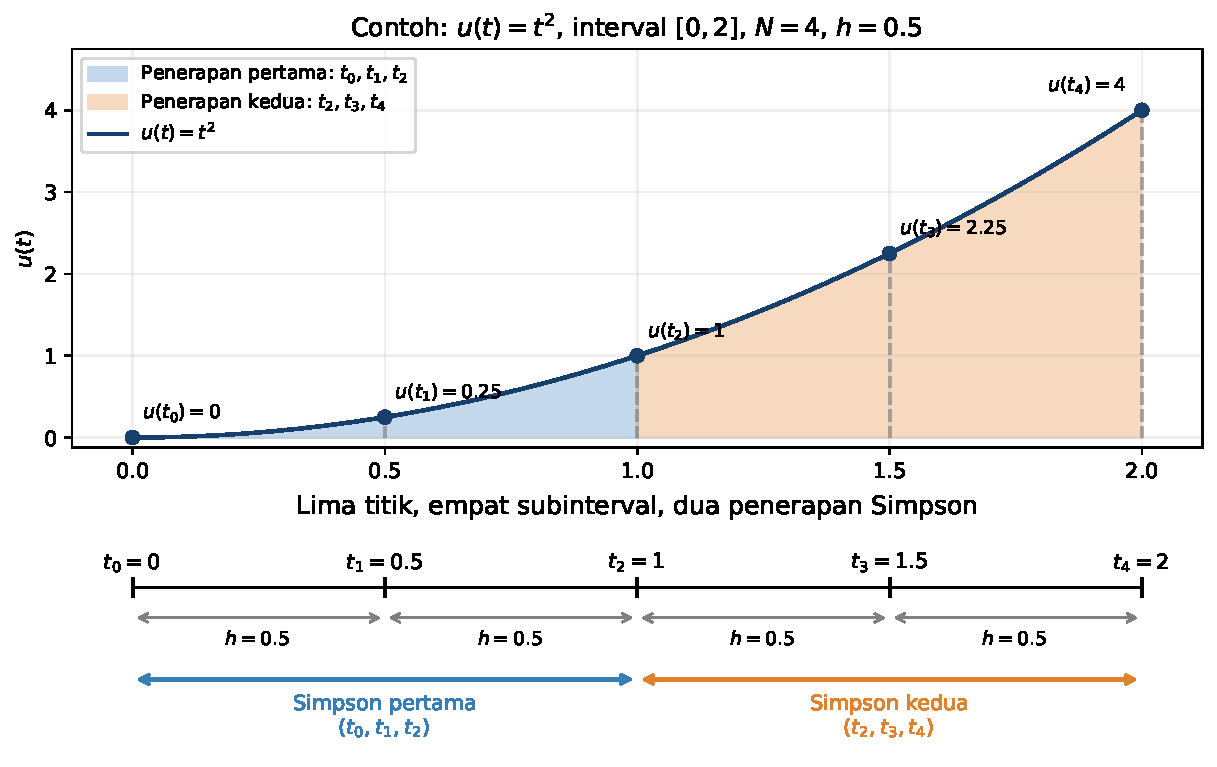
\includegraphics[width=0.95\linewidth]{Gambar/ilustrasi_simpson.pdf}
 \caption{Ilustrasi Simpson $1/3$ komposit untuk $u(t)=t^2$ pada $[0,2]$.
 Lima titik membentuk empat subinterval dengan lebar $h=0.5$.
 Daerah biru memakai tiga titik pertama dan daerah jingga memakai tiga
 titik terakhir. Nilai integral didekati dengan menjumlahkan luas keduanya.}
 \label{fig:ilustrasi-simpson}
\end{figure}
Karena fungsi ilustrasi sudah berbentuk parabola, pendekatan Simpson
berimpit dengan kurvanya. Untuk sinyal Gaussian dan trigonometri pada
soal, kurva pada setiap pasangan subinterval didekati dengan parabola;
karena itu perhitungan memerlukan pembagian interval yang lebih rapat.

Metode trapesium merupakan alternatif yang lebih sederhana. Untuk fungsi
yang cukup halus dan langkah yang cukup kecil, memperkecil $h$ menjadi
setengahnya umumnya memperkecil suku galat utama trapesium sekitar
empat kali dan Simpson sekitar enam belas kali \cite{mit_simpson}.
Hal ini menjelaskan alasan Simpson dipilih untuk integran halus pada
tugas ini. Besarnya galat tetap bergantung pada fungsi dan kerapatan
titik, terutama ketika sinyal berosilasi cepat. Kestabilan hasil diperiksa
dengan membandingkan dua tingkat kerapatan titik.
Implementasi menggunakan \texttt{scipy.integrate.simpson}
\cite{scipy_simpson}.

\section{Pembahasan}
\subsection{Representasi ortogonal dan deret Fourier}
Faktor Gaussian dan setiap faktor kosinus pada Persamaan~\eqref{eq:sinyal}
merupakan fungsi genap, sehingga $f(-t)=f(t)$. Akibatnya,
$\langle f,\sin(nt)\rangle=0$ dan $b_n=0$ untuk seluruh $n\geq1$.
Simetri ini menyederhanakan perhitungan koefisien kosinus menjadi
\[
 a_n=\frac2\pi\int_0^\pi f(t)\cos(nt)\,dt,\qquad n\geq0.
\]
Koefisien tersebut dihitung dengan aturan Simpson $1/3$ komposit
pada $[0,\pi]$, sesuai Persamaan~\eqref{eq:simpson}.
Untuk interval ini, batas bawahnya $a=0$ dan batas atasnya $b=\pi$.
Ambil $N=8192$ subinterval, sehingga $h=\pi/8192$ dan $t_j=jh$
untuk $j=0,1,\ldots,8192$. Titik pertama adalah $t_0=0$ dan titik
terakhir adalah $t_{8192}=\pi$. Fungsi di dalam integral adalah
$u(t)=f(t)\cos(nt)$ untuk setiap indeks $n$ yang sedang dihitung.
Koefisien numeriknya dihitung dengan
\[
 a_n\approx\frac2\pi Q_{8192,[0,\pi]}[f(t)\cos(nt)].
\]
Implementasi menggunakan \texttt{scipy.integrate.simpson}
\cite{scipy_simpson}, dengan koefisien dihitung sampai $n=100$.
Sebagai pemeriksaan simetri, integral koefisien sinus juga dievaluasi pada
$16385$ titik di $[-\pi,\pi]$. Nilai maksimum $|b_n|$ untuk
$1\leq n\leq100$ adalah \MaksSinus, yang mendekati nol pada
ketelitian komputer. Beberapa koefisien kosinus diberikan berikut ini.

\begin{table}[H]
 \centering
 \caption{Koefisien Fourier kosinus hasil integrasi numerik.}
 \label{tab:koefisien}
 \begin{tabular}{r|r}
  \hline
  $n$ & $a_n$ \\ \hline
  \inputrows{hasil_numerik/koefisien.tex}
 \end{tabular}
\end{table}
Koefisien terbesar berada di sekitar $n=2$, dengan kelompok koefisien
lain di sekitar $n=5$ dan $n=50$. Selubung Gaussian menyebabkan
representasi sinyal memerlukan koefisien pada frekuensi-frekuensi di
sekitar ketiga frekuensi pembentuknya.

Hubungan dengan proyeksi ortogonal dapat dijelaskan melalui subruang
\[
 V_K=\operatorname{span}\{1,\cos t,\sin t,\ldots,\cos(Kt),\sin(Kt)\}.
\]
Pada interval pengamatan, $\langle1,1\rangle=2\pi$ dan
$\langle\cos(nt),\cos(nt)\rangle=\pi$. Karena komponen sinus nol,
proyeksi ortogonal dinyatakan sebagai
\[
 P_{V_K}f(t)=\frac{\langle f,1\rangle}{2\pi}
 +\sum_{n=1}^{K}\frac{\langle f,\cos(nt)\rangle}{\pi}\cos(nt)
 =\frac{a_0}{2}+\sum_{n=1}^{K}a_n\cos(nt)=S_Kf(t).
\]
Artinya, koefisien yang dihitung secara numerik merupakan pendekatan
terhadap koefisien proyeksi ortogonal $f$ pada $V_K$.

\subsection{Aproksimasi dan konvergensi}
Menggunakan koefisien numerik pada pembahasan sebelumnya, dibentuk
jumlah parsial
\[
 S_Kf(t)=\frac{a_0}{2}+\sum_{n=1}^{K}a_n\cos(nt).
\]
Beberapa orde yang dibandingkan adalah $K=5$, $10$, $20$, $30$, $40$,
$50$, $60$, dan $100$. Galat setiap aproksimasi dihitung langsung dari
selisih sinyal pada $[-\pi,\pi]$, yaitu
\[
 \|f-S_Kf\|_2\approx
 \left(Q_{16384,[-\pi,\pi]}[|f(t)-S_Kf(t)|^2]\right)^{1/2}.
\]
Hasilnya ditampilkan pada Tabel~\ref{tab:galat}; integral galat tidak
dihitung menggunakan bentuk tertutup analitis.

\begin{table}[H]
 \centering
 \caption{Galat aproksimasi Fourier pada seluruh interval $[-\pi,\pi]$.}
 \label{tab:galat}
 \begin{tabular}{r|c}
  \hline
  $K$ & $\|f-S_Kf\|_2$ \\ \hline
  \inputrows{hasil_numerik/galat.tex}
 \end{tabular}
\end{table}
Untuk $K=5$, galat masih sekitar $0.28948616$. Pada $K=10$ hingga
$40$, galat hampir tetap di sekitar $0.188278$, karena basis yang dipakai
belum mencakup komponen di sekitar frekuensi $50$. Pada $K=50$, galat
menurun menjadi sekitar $0.08808327$. Setelah frekuensi-frekuensi di
sekitar $50$ ikut disertakan, galat turun menjadi sekitar
$5.5873\times10^{-5}$ pada $K=60$ dan $1.2057\times10^{-5}$ pada $K=100$.

\begin{figure}[H]
 \centering
 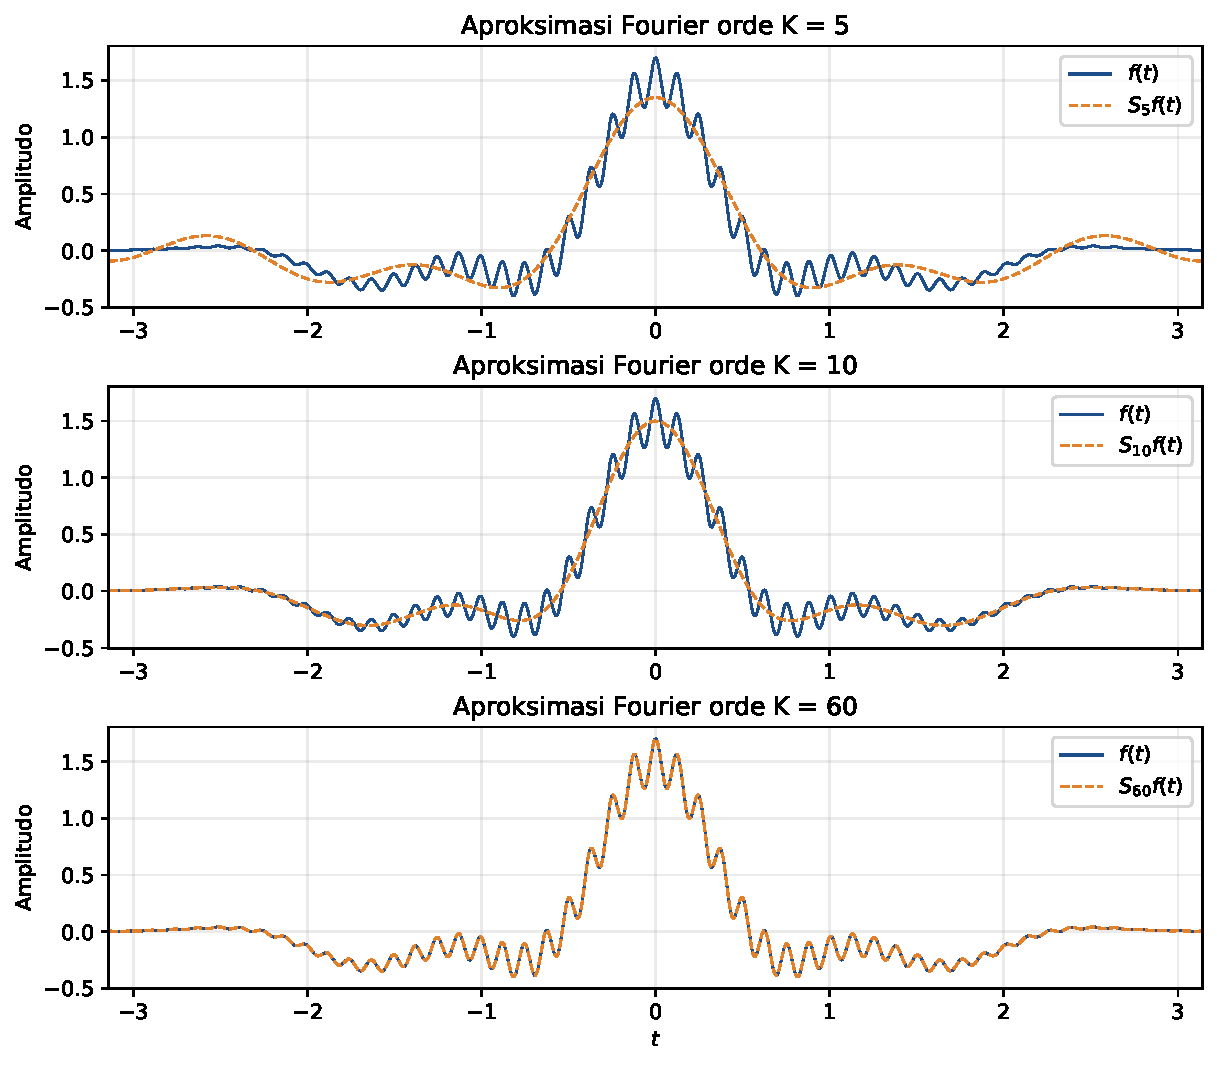
\includegraphics[width=0.85\linewidth]{Gambar/aproksimasi_numerik.pdf}
 \caption{Perbandingan numerik $f$ dan $S_Kf$ pada $[-\pi,\pi]$
 untuk $K=5$, $10$, dan $60$.}
 \label{fig:aproksimasi}
\end{figure}
\begin{figure}[H]
 \centering
 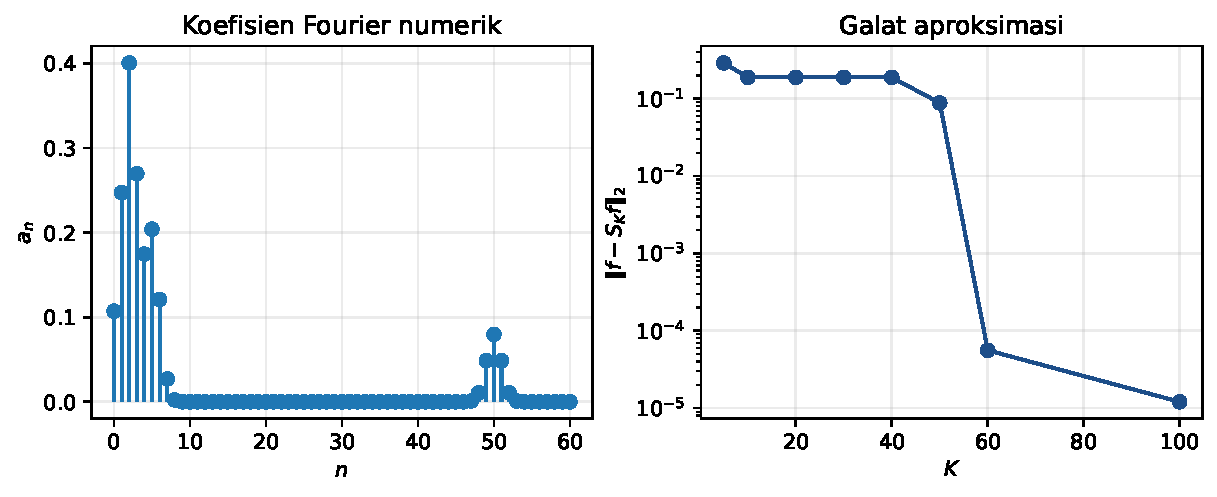
\includegraphics[width=0.95\linewidth]{Gambar/koefisien_galat_numerik.pdf}
 \caption{Koefisien Fourier dan perubahan galat aproksimasi ketika
 $K$ bertambah. Galat ditampilkan pada skala logaritmik.}
 \label{fig:koefisien-galat}
\end{figure}
Penurunan galat sesuai dengan sifat aproksimasi terbaik. Dengan koefisien
eksak, $S_Kf=P_{V_K}f$ meminimumkan galat terhadap semua fungsi dalam
$V_K$. Karena $V_K\subseteq V_{K+1}$, berlaku
\[
 \|f-S_{K+1}f\|_2\leq\|f-S_Kf\|_2.
\]
Kelengkapan sistem trigonometri juga memberikan konvergensi
$\|f-S_Kf\|_2\to0$ ketika $K\to\infty$. Tabel dan grafik menunjukkan
perilaku yang sesuai dengan sifat tersebut untuk orde yang diperiksa.
Pada $K=60$, kurva jumlah parsial hampir berimpit dengan sinyal asli,
termasuk osilasi cepatnya.

\subsection{Transformasi Fourier dan analisis spektral}
Tuliskan $g(t)=e^{-t^2/2}$ dan pisahkan sinyal menjadi
\[
 f(t)=f_1(t)+f_2(t)+f_3(t),
\]
dengan $f_1(t)=g(t)\cos(2t)$, $f_2(t)=\tfrac12g(t)\cos(5t)$,
dan $f_3(t)=0.2g(t)\cos(50t)$. Sesuai pasangan transformasi pada soal,
$g$ memiliki spektrum Gaussian. Dengan linearitas dan sifat modulasi,
setiap faktor kosinus menggeser spektrum $g$ ke dua sisi frekuensi.
Hubungan transformasinya dapat diringkas sebagai
\begin{equation}
 \begin{aligned}
 \widehat f_\varepsilon(\omega)={}&
 \frac12[\widehat g(\omega-2)+\widehat g(\omega+2)]\\
 &+\frac14[\widehat g(\omega-5)+\widehat g(\omega+5)]\\
 &+\frac{\varepsilon}{2}[\widehat g(\omega-50)+\widehat g(\omega+50)].
 \end{aligned}
 \label{eq:modulasi}
\end{equation}
Hubungan ini menjelaskan letak komponen spektrum, sedangkan nilai-nilai
transformasi berikut diperoleh dari integrasi numerik.

Untuk mendekati domain $\mathbb R$, digunakan batas waktu $[-8,8]$,
$N=16384$ subinterval, dan $\Delta t=0.0009765625$.
Karena $f$ real dan genap, nilai transformasi dihitung dengan
\begin{equation}
 \widetilde{\widehat f}(\omega)=\frac2{\sqrt{2\pi}}
 Q_{8192,[0,8]}[f(t)\cos(\omega t)].
 \label{eq:transformasi-numerik}
\end{equation}
Sebagai pemeriksaan sifat modulasi, $\widehat g$ pada
Persamaan~\eqref{eq:modulasi} juga dihitung dengan aturan Simpson
menggunakan fungsi $g(t)$. Pada $\omega=0$, $2$, $5$, dan $50$,
selisih maksimum hasil penjumlahan transformasi yang digeser dengan
integrasi langsung $f$ adalah \GalatModulasi.

Grid spektrum menggunakan $\omega\in[-60,60]$ dengan
$\Delta\omega=0.01$. Magnitudo dan kerapatan energi dihitung dari
$|\widetilde{\widehat f}(\omega)|$ dan
$|\widetilde{\widehat f}(\omega)|^2$, lalu digambarkan pada
Gambar~\ref{fig:spektrum}. Puncak positif dicari pada grid di
rentang $[1,3]$, $[4,6]$, dan $[49,51]$.

\begin{figure}[H]
 \centering
 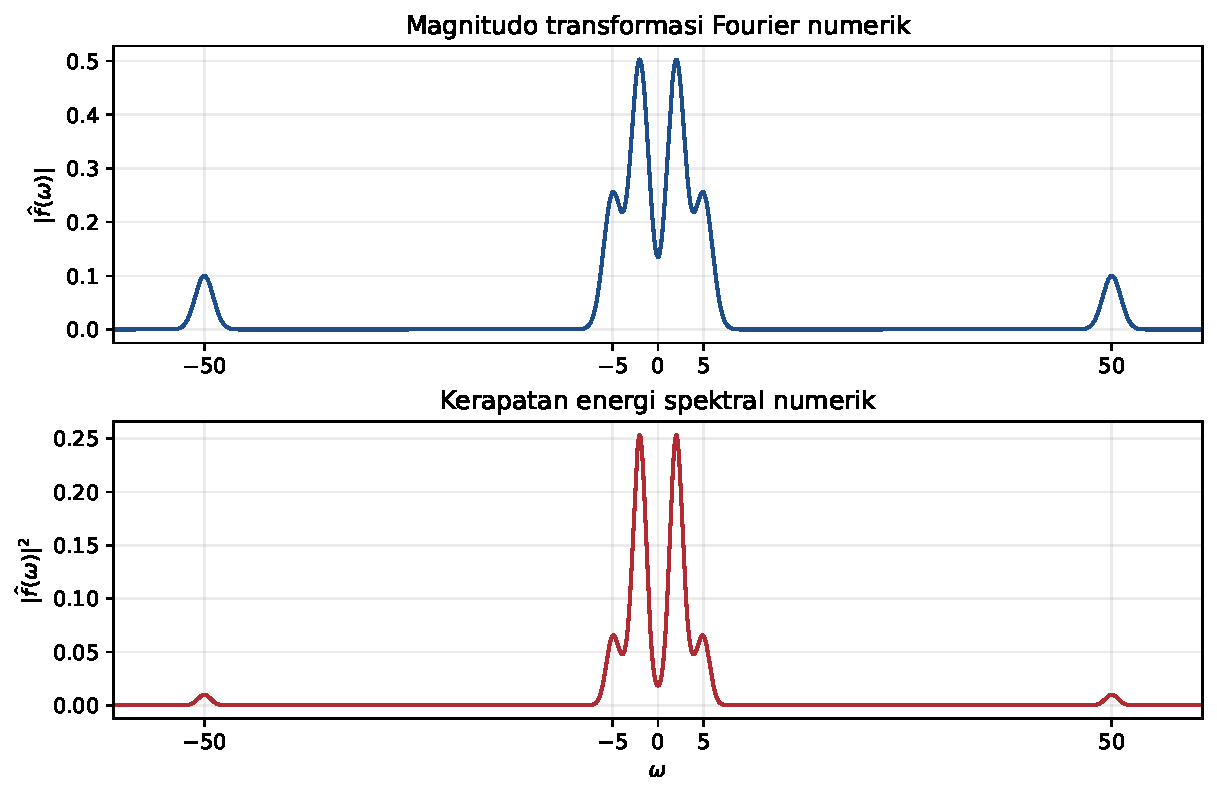
\includegraphics[width=0.9\linewidth]{Gambar/spektrum_numerik.pdf}
 \caption{Magnitudo dan kerapatan energi spektral hasil integrasi numerik.}
 \label{fig:spektrum}
\end{figure}
\begin{table}[H]
 \centering
 \caption{Puncak spektrum pada sisi frekuensi positif, dengan resolusi grid $0.01$.}
 \label{tab:puncak}
 \begin{tabular}{c|c|c}
  \hline
  $\omega$ pada grid & $|\widehat f(\omega)|$ & $|\widehat f(\omega)|^2$ \\ \hline
  \inputrows{hasil_numerik/puncak.tex}
 \end{tabular}
\end{table}
Dua komponen utama berasal dari frekuensi pembentuk $\omega_1=2$ dan
$\omega_2=5$. Pada spektrum gabungan, puncak positifnya terdeteksi di
sekitar $2.02$ dan $4.92$. Pergeseran kecil dari $2$ dan $5$ terjadi
karena spektrum kedua komponen saling bertumpang tindih. Puncak
tertinggi berada di sekitar $\omega=\pm2$, sehingga komponen pertama
merupakan komponen dominan. Gangguan frekuensi tinggi berasal dari
$\omega_3=50$ dan tampak sebagai kelompok puncak di sekitar $\omega=\pm50$,
dengan magnitudo sekitar $0.1$ serta kerapatan energi sekitar $0.01$.
Frekuensi pembentuk tertinggi dan komponen dengan magnitudo tertinggi
merupakan dua informasi yang berbeda.

Pengaruh $\varepsilon$ diperiksa dengan menghitung ulang sinyal untuk
$\varepsilon=0.1$, $0.2$, dan $0.4$, sementara frekuensi-frekuensinya tetap.
Tabel~\ref{tab:epsilon} dan Gambar~\ref{fig:epsilon} menunjukkan perubahan
spektrum di sekitar frekuensi $50$.
\begin{table}[H]
 \centering
 \caption{Pengaruh $\varepsilon$ terhadap komponen frekuensi tinggi.}
 \label{tab:epsilon}
 \begin{tabular}{c|c|c}
  \hline
  $\varepsilon$ & $|\widehat f_\varepsilon(50)|$ & $|\widehat f_\varepsilon(50)|^2$ \\ \hline
  \inputrows{hasil_numerik/epsilon.tex}
 \end{tabular}
\end{table}
\begin{figure}[H]
 \centering
 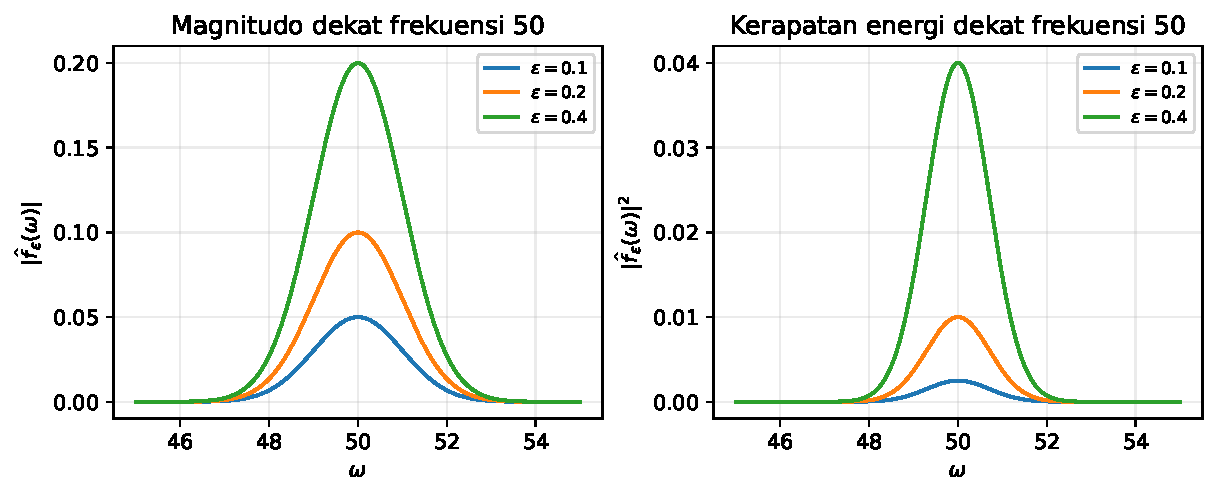
\includegraphics[width=0.95\linewidth]{Gambar/epsilon_numerik.pdf}
 \caption{Perubahan magnitudo dan kerapatan energi di sekitar
 $\omega=50$ ketika $\varepsilon$ berubah. Sisi negatif memiliki bentuk simetris.}
 \label{fig:epsilon}
\end{figure}
Ketika $\varepsilon$ naik dua kali lipat, magnitudo puncak frekuensi tinggi
naik sekitar dua kali lipat dan kerapatan energinya naik sekitar empat
kali lipat. Letak kelompok spektrum frekuensi tinggi tetap di sekitar
$\pm50$. Dengan demikian, $\varepsilon$ mengatur kekuatan gangguan,
sedangkan $\omega_3$ mengatur frekuensinya.

Untuk menentukan waktu ketika komponen frekuensi tertinggi paling kuat,
$|f_3(t)|$ dievaluasi pada seluruh $16385$ titik grid di $[-\pi,\pi]$.
Pencarian maksimum numerik memberikan
\[
 \boxed{t_*=0.000000,\qquad |f_3(t_*)|=0.200000.}
\]
Evaluasi sinyal total pada titik tersebut memberikan $f(0)=1.7$.
Grafik sinyal dan komponen gangguannya ditampilkan berikut ini.
\begin{figure}[H]
 \centering
 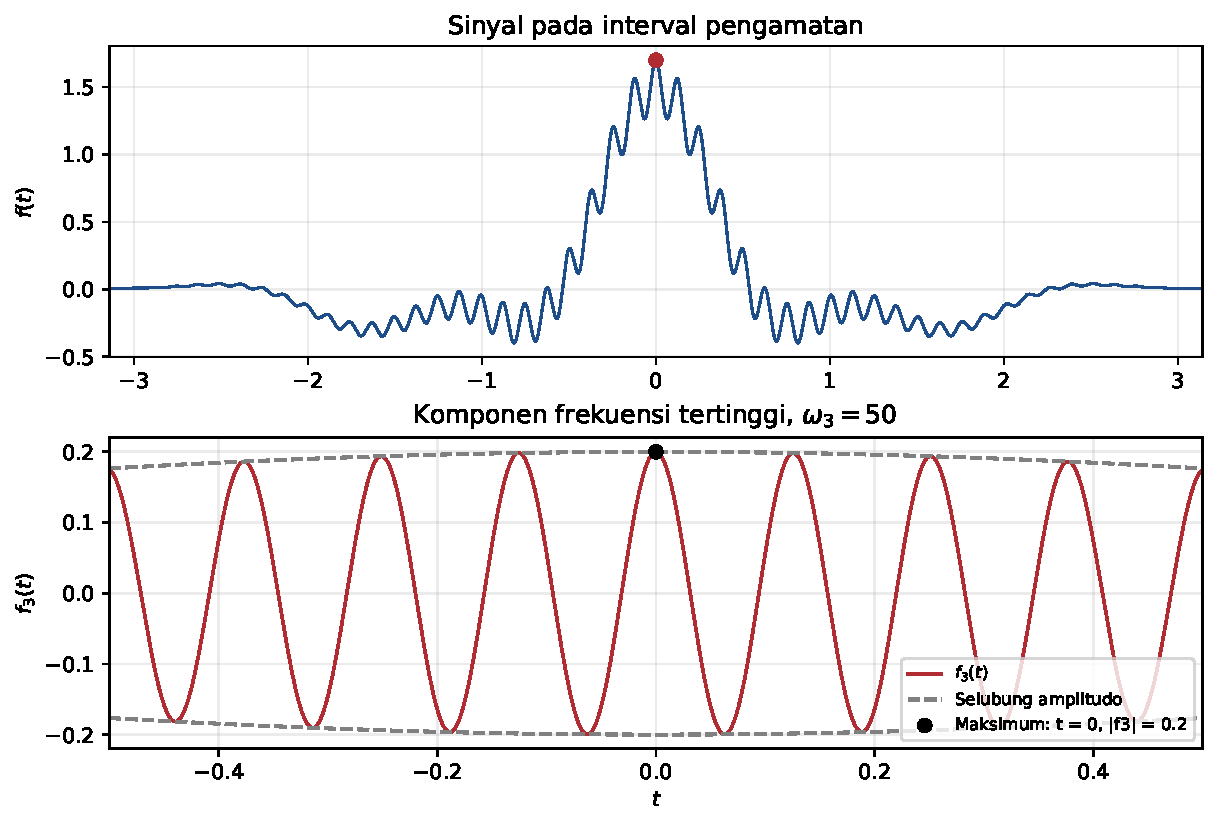
\includegraphics[width=0.9\linewidth]{Gambar/sinyal_numerik.pdf}
 \caption{Sinyal pada interval pengamatan dan pembesaran komponen
 berfrekuensi $50$, dengan penanda maksimum amplitudo pada $t=0$.}
 \label{fig:sinyal}
\end{figure}
Komponen ini memiliki frekuensi tetap $50$ sepanjang waktu; $t=0$
menyatakan waktu amplitudonya paling besar. Transformasi Fourier global
tidak memasangkan satu frekuensi dengan satu waktu tertentu.
Jika waktu yang dimaksud adalah waktu satu osilasi, periode faktor
kosinusnya adalah
\[
 T_3=\frac{2\pi}{50}\approx0.125664\ \text{satuan waktu}.
\]
Periode ini berlaku untuk $\cos(50t)$, sedangkan $f_3(t)$ secara keseluruhan
tidak periodik karena selubung Gaussiannya berubah terhadap waktu.

\subsection{Analisis komparatif}
Deret Fourier dan transformasi Fourier memberikan informasi yang saling
melengkapi. Deret Fourier merepresentasikan periodisasi sinyal pada
$[-\pi,\pi]$ menggunakan frekuensi diskret $n\in\mathbb Z$. Koefisiennya
menunjukkan kontribusi setiap basis trigonometri, dan jumlah parsialnya
menunjukkan seberapa baik sinyal dapat didekati oleh subruang Fourier
berdimensi terbatas. Hasil numerik memperlihatkan kelompok koefisien
utama di sekitar $n=2$ dan $n=5$, serta kelompok gangguan di sekitar $n=50$.

Transformasi Fourier merepresentasikan sinyal asli pada $\mathbb R$
menggunakan frekuensi kontinu $\omega$. Grafik magnitudo menunjukkan
lokasi dan kekuatan komponen spektrum, sedangkan kuadrat magnitudo
menunjukkan distribusi energi terhadap frekuensi. Kelompok spektrum di
sekitar $\pm2$ dan $\pm5$ mengenali dua komponen utama; kelompok yang
terpisah di sekitar $\pm50$ mengenali gangguan berfrekuensi tinggi.
Besarnya magnitudo kelompok pertama menunjukkan bahwa komponen pada
frekuensi $2$ paling dominan.

Selubung Gaussian membuat representasi frekuensi setiap komponen
menyebar di sekitar frekuensi pembentuknya. Karena itu, koefisien deret
bukan hanya terdapat pada $n=2$, $5$, dan $50$. Hal yang sama menjelaskan
mengapa $S_{50}f$ belum menangkap seluruh gangguan, sedangkan $S_{60}f$
menunjukkan galat yang jauh lebih kecil. Pengamatan deret dibatasi pada
satu periode hasil periodisasi; transformasi menggambarkan sinyal asli
yang amplitudonya meluruh pada domain waktu yang tidak terbatas.

Kesamaan Parseval menghubungkan energi pada satu periode dengan
penjumlahan kuadrat koefisien diskret. Teorema Plancherel menghubungkan
energi sinyal asli dengan integral kerapatan energi kontinu. Perbandingan
nilai energi kedua pendekatan dilakukan pada pembahasan berikut dengan
normalisasi transformasi yang sama seperti pada dasar teori.

\subsection{Analisis Komparatif}
Untuk memeriksa Parseval secara numerik, energi pada interval pengamatan
dihitung melalui aturan Simpson:
\[
 E_{[-\pi,\pi]}:=\int_{-\pi}^{\pi}|f(t)|^2\,dt
 \approx\EnergiInterval.
\]
Energi dari koefisien hingga orde $K$ dihitung sebagai
\[
 E_K=\pi\left[\frac{a_0^2}{2}+\sum_{n=1}^{K}(a_n^2+b_n^2)\right].
\]
Koefisien sinus numerik mendekati nol. Tabel~\ref{tab:parseval}
memperlihatkan energi jumlah parsial, galat aproksimasi, dan selisih
energi relatif $|E_{[-\pi,\pi]}-E_K|/E_{[-\pi,\pi]}$.

\begin{table}[H]
 \centering
 \caption{Pemeriksaan numerik kesamaan Parseval dengan jumlah koefisien terbatas.}
 \label{tab:parseval}
 \begin{tabular}{r|c|c|c}
  \hline
  $K$ & $\|f-S_Kf\|_2$ & $E_K$ & Selisih energi relatif \\ \hline
  \inputrows{hasil_numerik/parseval.tex}
 \end{tabular}
\end{table}
Pada $K=100$, energi koefisien adalah $E_{100}\approx\EnergiParseval$,
dengan selisih absolut dari energi waktu sebesar \GalatParseval.
Dengan koefisien eksak, selisih energi jumlah parsial sama dengan
$\|f-S_Kf\|_2^2$. Nilai numerik dalam tabel sesuai dengan hubungan
tersebut pada ketelitian perhitungan. Selisih yang tersisa berasal dari
koefisien yang belum disertakan serta galat kuadratur dan pembulatan.
Karena penjumlahan hanya sampai $K=100$, hasilnya merupakan pemeriksaan
numerik jumlah parsial terhadap Parseval.

Untuk Plancherel, normalisasi uniter pada Persamaan~\eqref{eq:konvensi}
digunakan secara konsisten, sehingga tidak diperlukan faktor tambahan
$1/(2\pi)$ pada integral energi spektral. Energi waktu dan energi frekuensi
dihitung secara terpisah dengan Simpson:
\begin{align*}
 E_t^{(8)}&:=\int_{-8}^{8}|f(t)|^2\,dt\approx\EnergiWaktu,\\
 E_\omega^{(60)}&:=\int_{-60}^{60}
 |\widetilde{\widehat f}(\omega)|^2\,d\omega\approx\EnergiFrekuensi.
\end{align*}
Hasil penghalusan grid ditampilkan pada Tabel~\ref{tab:plancherel}.
\begin{table}[H]
 \centering
 \caption{Pemeriksaan numerik Plancherel pada batas waktu $[-8,8]$
 dan batas frekuensi $[-60,60]$.}
 \label{tab:plancherel}
 \small
 \begin{tabular}{r|c|c|c|c}
  \hline
  $N$ & $\Delta\omega$ & $E_t^{(8)}$ & $E_\omega^{(60)}$ & Selisih absolut \\ \hline
  \inputrows{hasil_numerik/plancherel.tex}
 \end{tabular}
\end{table}
Selisih absolut energi waktu dan frekuensi adalah \GalatPlancherel,
dengan selisih relatif \GalatRelPlancherel. Nilai ini menunjukkan
kesesuaian kedua perhitungan pada ketelitian komputer, bukan batas galat
terhadap integral eksak di seluruh $\mathbb R$.
Perubahan batas waktu dari $[-6,6]$ menjadi $[-8,8]$ tidak mengubah
energi pada angka yang dilaporkan. Untuk koefisien deret, penghalusan
grid dari $8192$ menjadi $16384$ subinterval pada $[-\pi,\pi]$
memberikan perubahan maksimum koefisien kosinus sebesar \BedaKoefisien.

\begin{figure}[H]
 \centering
 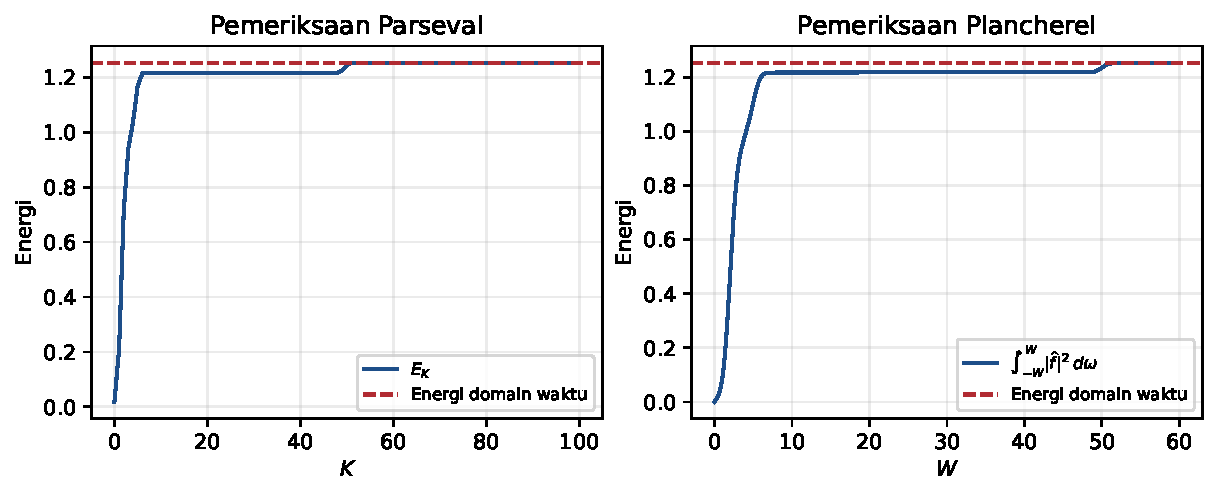
\includegraphics[width=0.95\linewidth]{Gambar/energi_numerik.pdf}
 \caption{Energi kumulatif koefisien deret dan energi kumulatif spektrum.
 Garis putus-putus menunjukkan energi waktu pada masing-masing domain.}
 \label{fig:energi}
\end{figure}
Energi pengamatan dan energi seluruh sinyal berbeda sekitar
$6.2805\times10^{-6}$. Perbedaan ini berasal dari energi sinyal di luar
$[-\pi,\pi]$, yang ikut dihitung pada pendekatan Plancherel.
Dengan demikian, kedua kesamaan energi berlaku untuk objek yang berbeda:
Parseval pada satu periode dari sinyal yang diperiodisasi, dan Plancherel
pada sinyal asli di seluruh domain waktu.

Dari keseluruhan hasil, dua komponen utama dikenali melalui kelompok
koefisien dan spektrum di sekitar frekuensi $2$ serta $5$. Gangguan
berfrekuensi tinggi dikenali melalui kelompok yang terpisah di sekitar
$50$, penurunan galat ketika orde aproksimasi melewati frekuensi tersebut,
dan peningkatan energi spektralnya saat $\varepsilon$ bertambah.

\section{Kesimpulan}
Koefisien Fourier dihitung secara numerik dengan memanfaatkan simetri
genap sinyal. Koefisien sinus mendekati nol, sedangkan koefisien kosinus
membentuk kelompok di sekitar $n=2$, $5$, dan $50$. Jumlah parsial
merupakan pendekatan numerik terhadap proyeksi ortogonal pada subruang
trigonometri. Galat $L^2$ tidak meningkat pada orde yang diperiksa dan
menurun menjadi sekitar $5.5873\times10^{-5}$ pada $K=60$, sesuai
sifat aproksimasi terbaik dan konvergensi dalam $L^2$.

Transformasi Fourier numerik, yang konsisten dengan linearitas dan
modulasi spektrum Gaussian, menunjukkan dua komponen utama di sekitar
$\omega=\pm2$ dan $\pm5$, dengan komponen pertama paling dominan.
Gangguan berfrekuensi tinggi berada di sekitar $\omega=\pm50$.
Peningkatan $\varepsilon$ memperbesar magnitudo serta kerapatan energi
gangguan. Komponen berfrekuensi $50$ paling kuat pada $t=0$, dengan
amplitudo $0.2$ dan periode faktor kosinus sekitar $0.125664$ satuan waktu.

Pemeriksaan Parseval memberikan energi pengamatan \EnergiInterval,
sedangkan energi koefisien sampai $K=100$ adalah \EnergiParseval.
Pemeriksaan Plancherel memberikan energi waktu dan energi frekuensi
sekitar \EnergiWaktu. Selisih yang kecil pada masing-masing pemeriksaan
mendukung kesesuaian representasi energi dalam perhitungan numerik.
Perbedaan energi antarpendekatan berasal dari perbedaan domain waktu.
Dengan demikian, deret Fourier dan transformasi Fourier dapat mengenali
komponen utama serta gangguan melalui lokasi frekuensi, besar koefisien
atau magnitudo, dan kontribusi energinya.

\bibliographystyle{plain}
\bibliography{ref}
\end{document}

